\chapter{Release 4:Système de Réunions Vidéo}

\DeclareRobustCommand{\greencheck}{%
  \tikz\fill[scale=0.4, color=green]
  (0,.35) -- (.25,0) -- (1,.7) -- (.25,.15) -- cycle;%
}

\minitoc
\section*{Introduction}
\addcontentsline{toc}{section}{Introduction}
Dans le cadre de la sixième phase du développement de notre application, nous avons concentré nos efforts sur l'implémentation d'un système complet de réunions vidéo. Cette fonctionnalité permet aux utilisateurs de créer, planifier, gérer et participer à des réunions en ligne directement depuis la plateforme. Ce module constitue une extension majeure de nos services, renforçant significativement les capacités de collaboration à distance entre les utilisateurs.

\section{Objectifs du Sprint 6}

\subsection{Système de Réunions Vidéo}
L'objectif principal de ce sprint est de développer un module de visioconférence intégré à notre plateforme. Ce système doit permettre aux utilisateurs de créer des réunions avec différentes configurations, d'inviter d'autres membres, de gérer le déroulement des sessions et d'accéder à l'historique des réunions passées. Les fonctionnalités avancées incluent l'enregistrement des sessions, le partage de présentations et la consultation de statistiques. L'ensemble du module vise à offrir une expérience fluide et performante pour les réunions professionnelles à distance, renforçant ainsi l'écosystème collaboratif de notre application.

\section{Backlog Fonctionnel – Sprint 6}

\subsection{Backlog Produit – Système de Réunions}
Le tableau ci-dessous recense les user stories associées au système de réunions vidéo. Ces fonctionnalités ont été priorisées selon trois niveaux (Haute, Moyenne, Basse) selon leur impact sur le fonctionnement de l'application.

\usepackage{tabularx}
\usepackage{float}
\usepackage{caption}

\begin{table}[H]
\centering
\begin{tabularx}{\textwidth}{|c|X|c|}
\hline
\textbf{User Story} & \textbf{Description} & \textbf{Priorité} \\
\hline
US-01 & En tant qu'utilisateur, je veux pouvoir créer des réunions vidéo avec un titre, une description et une durée. & Haute \\
\hline
US-02 & En tant qu'utilisateur, je veux pouvoir inviter d'autres utilisateurs à mes réunions. & Haute \\
\hline
US-03 & En tant qu'utilisateur, je veux pouvoir démarrer une réunion que j'ai créée. & Haute \\
\hline
US-04 & En tant qu'utilisateur, je veux pouvoir rejoindre une réunion à laquelle je suis invité. & Haute \\
\hline
US-05 & En tant qu'utilisateur, je veux pouvoir mettre fin à une réunion que j'ai créée. & Haute \\
\hline
US-06 & En tant qu'utilisateur, je veux pouvoir activer ou désactiver l'enregistrement de mes réunions. & Moyenne \\
\hline
US-07 & En tant qu'utilisateur, je veux pouvoir spécifier un type de réunion (one-on-one, groupe, projet). & Moyenne \\
\hline
US-08 & En tant qu'utilisateur, je veux pouvoir voir la liste de mes réunions planifiées et passées. & Haute \\
\hline
US-09 & En tant qu'utilisateur, je veux pouvoir ajouter une présentation à ma réunion. & Moyenne \\
\hline
US-10 & En tant qu'utilisateur, je veux pouvoir consulter les statistiques sur mes réunions (participants, durée, etc.). & Basse \\
\hline
US-11 & En tant qu'utilisateur, je veux pouvoir consulter l'historique de mes réunions passées. & Moyenne \\
\hline
US-12 & En tant qu'utilisateur, je veux pouvoir accéder aux enregistrements de mes réunions passées. & Moyenne \\
\hline
US-13 & En tant qu'utilisateur, je veux recevoir des notifications pour les invitations à des réunions. & Haute \\
\hline
US-14 & En tant qu'utilisateur, je veux recevoir des rappels pour mes réunions à venir. & Moyenne \\
\hline
\end{tabularx}
\caption{User Stories liées au système de réunions vidéo}
\end{table}

\section{Raffinement des cas d'utilisation}
Nous avons procédé au raffinement des cas d'utilisation afin de mieux comprendre et structurer les interactions entre les acteurs et les fonctionnalités du système. Cette étape nous a permis de passer d'une vision globale à une représentation plus précise, notamment à travers l'élaboration de diagrammes UML.

\subsection{Raffinement des cas d'utilisation - Système de Réunions}
\subsubsection{Raffinement du cas d'utilisation "Créer une réunion"}
La figure 6.1 présente le raffinement du cas d'utilisation "Créer une réunion", suivie par sa description textuelle dans le tableau 6.2.

% Insérer ici l'image du diagramme de cas d'utilisation
\begin{figure}[H]
    \centering
    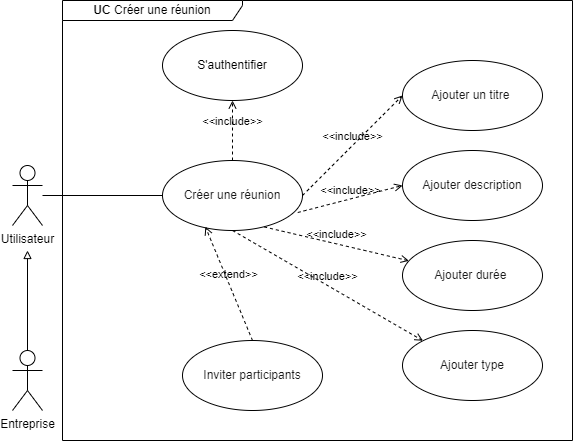
\includegraphics[width=0.8\textwidth]{images/Créeruneréunionfinale.drawio.png}
    \caption{Diagramme de cas d'utilisation Créer une réunion}
    \label{fig:créer_une_réunion}
\end{figure}

\begin{table}[H]
\centering
\begin{tabular}{|p{4cm}|p{10cm}|}
\hline
\textbf{Élément} & \textbf{Description} \\ \hline
Cas d'utilisation & Créer une réunion \\ \hline
Acteur & Utilisateur \\ \hline
Précondition & L'utilisateur est authentifié dans le système. \\ \hline
Postcondition & La réunion est créée et les invitations sont envoyées aux participants. \\ \hline
Scénario nominal & 
1. L'utilisateur s'authentifie. \newline
2. L'utilisateur accède à la section de réunions. \newline
3. L'utilisateur sélectionne "Créer une nouvelle réunion". \newline
4. L'utilisateur remplit les champs requis (titre, description, date, heure, durée). \newline
5. L'utilisateur spécifie le type de réunion (one-on-one, groupe, projet). \newline
6. L'utilisateur invite d'autres participants. \newline
7. L'utilisateur peut ajouter des documents ou une présentation. \newline
8. L'utilisateur active ou désactive l'option d'enregistrement. \newline
9. L'utilisateur confirme la création de la réunion. \newline
10. Le système crée la réunion et envoie les invitations. \newline
11. L'utilisateur reçoit une confirmation de création. \\ \hline
Scénario alternatif & 
4a. Si des champs obligatoires sont incomplets, le système affiche un message d'erreur et invite à compléter les informations manquantes. \newline
6a. Si un utilisateur invité n'existe pas, le système affiche un message d'erreur. \newline
7a. Si la taille des documents dépasse la limite autorisée, le système informe l'utilisateur et demande de réduire la taille ou de changer les fichiers. \\ \hline
\end{tabular}
\caption{Description textuelle du cas d'utilisation Créer une réunion}
\end{table}

\subsubsection{Raffinement du cas d'utilisation "Rejoindre une réunion"}
La figure 6.2 présente le raffinement du cas d'utilisation "Rejoindre une réunion", suivie par sa description textuelle dans le tableau 6.3.

% Insérer ici l'image du diagramme de cas d'utilisation
\begin{figure}[H]
    \centering
    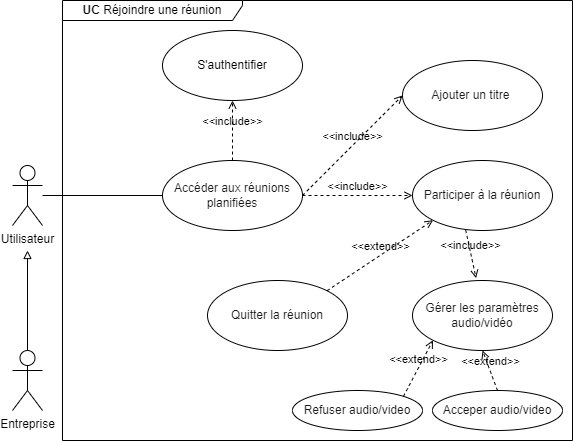
\includegraphics[width=0.8\textwidth]{images/RejoindreuneréunionV0finale.drawio.png}
    \caption{Diagramme de cas d'utilisation Rejoindre une réunion}
    \label{fig:régoindre_une_réunion}
\end{figure}
\begin{table}[H]
\centering
\begin{tabular}{|p{4cm}|p{10cm}|}
\hline
\textbf{Élément} & \textbf{Description} \\ \hline
Cas d'utilisation & Rejoindre une réunion \\ \hline
Acteur & Utilisateur \\ \hline
Précondition & L'utilisateur est authentifié et invité à une réunion active. \\ \hline
Postcondition & L'utilisateur rejoint la réunion et peut participer à la session vidéo. \\ \hline
Scénario nominal & 
1. L'utilisateur s'authentifie. \newline
2. L'utilisateur accède à la section de réunions. \newline
3. L'utilisateur consulte la liste de ses réunions planifiées. \newline
4. L'utilisateur sélectionne une réunion active. \newline
5. L'utilisateur clique sur "Rejoindre la réunion". \newline
6. Le système connecte l'utilisateur à la session vidéo. \newline
7. L'utilisateur peut activer/désactiver sa caméra et son microphone. \newline
8. L'utilisateur participe à la réunion. \\ \hline
Scénario alternatif & 
4a. Si la réunion n'a pas encore commencé, le système affiche un message indiquant que la réunion n'est pas encore active. \newline
6a. Si l'utilisateur rencontre des problèmes de connexion, le système propose des options de dépannage. \\ \hline
\end{tabular}
\caption{Description textuelle du cas d'utilisation Rejoindre une réunion}
\end{table}

\subsubsection{Raffinement du cas d'utilisation "Gérer les enregistrements de réunions"}
La figure 6.3 présente le raffinement du cas d'utilisation "Gérer les enregistrements de réunions", suivie par sa description textuelle dans le tableau 6.4.

% Insérer ici l'image du diagramme de cas d'utilisation
\begin{figure}[H]
    \centering
    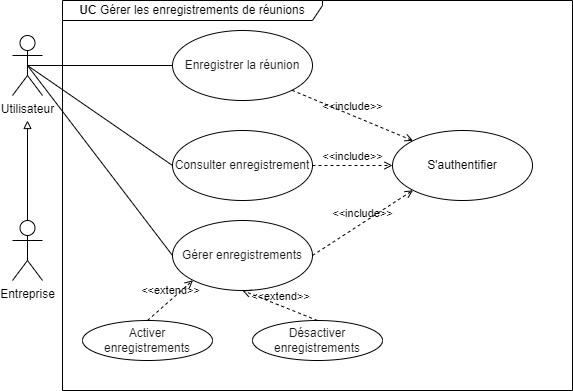
\includegraphics[width=0.8\textwidth]{images/Gérer les enregistrements de réunionsfinale.drawio.png}
    \caption{Diagramme de cas d'utilisation Gérer les enregistrements de réunions}
    \label{fig:gérer_enregistrement_réunion}
\end{figure}
\begin{table}[H]
\centering
\begin{tabular}{|p{4cm}|p{10cm}|}
\hline
\textbf{Élément} & \textbf{Description} \\ \hline
Cas d'utilisation & Gérer les enregistrements de réunions \\ \hline
Acteur & Utilisateur (créateur de la réunion) \\ \hline
Précondition & L'utilisateur est authentifié et a créé au moins une réunion. \\ \hline
Postcondition & L'enregistrement de la réunion est activé, désactivé ou consulté selon l'action choisie. \\ \hline
Scénario nominal & 
1. L'utilisateur s'authentifie. \newline
2. L'utilisateur accède à la section de réunions. \newline
3. L'utilisateur peut : \newline
\hspace{0.5cm} a. Activer l'enregistrement avant ou pendant une réunion. \newline
\hspace{0.5cm} b. Désactiver l'enregistrement pendant une réunion. \newline
\hspace{0.5cm} c. Consulter la liste des enregistrements de réunions passées. \newline
\hspace{0.5cm} d. Visionner un enregistrement spécifique. \newline
\hspace{0.5cm} e. Télécharger un enregistrement. \newline
\hspace{0.5cm} f. Supprimer un enregistrement. \newline
4. Le système exécute l'action demandée. \newline
5. L'utilisateur reçoit une confirmation de l'action effectuée. \\ \hline
\end{tabular}

\label{tab:gerer_enregistrements_part1}
\end{table}
\begin{table}[H]
\centering
\begin{tabular}{|p{4cm}|p{10cm}|}
\hline

Scénario alternatif & 
3c. Si aucun enregistrement n'existe, le système affiche un message approprié. \newline
3d. Si l'enregistrement est en cours de traitement, le système informe l'utilisateur du délai d'attente. \\ \hline
\end{tabular}
\caption{Cas d'utilisation \og Gérer les enregistrements de réunions \fg{}}
\label{tab:gerer_enregistrements_part2}
\end{table}


\section{Diagrammes de séquence}
Le diagramme de séquence est un type de diagramme UML qui modélise les interactions entre différents objets ou acteurs d'un système au cours du temps. Dans ce qui suit, nous allons dresser les diagrammes de séquences des cas d'utilisation raffinés précédemment.

\subsection{Diagrammes de séquence - Système de Réunions}
\subsubsection{Diagramme de séquence de "Créer une réunion"}
La figure 6.4 présente le diagramme de séquence du cas d'utilisation "Créer une réunion".

% Insérer ici l'image du diagramme de séquence
\begin{figure}[H]
    \centering
    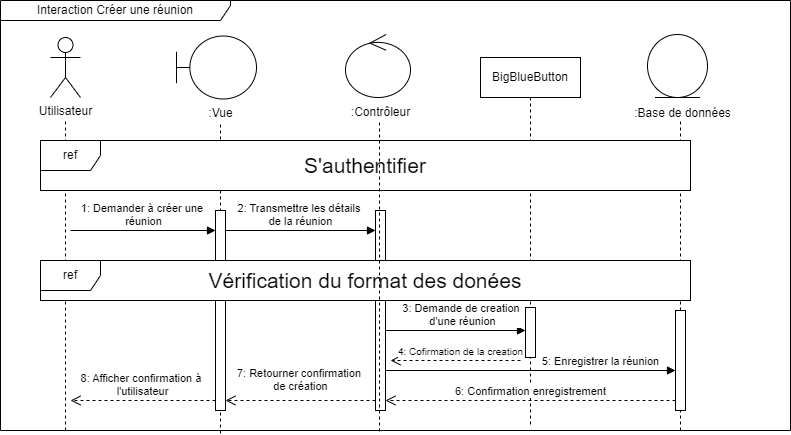
\includegraphics[width=0.8\textwidth]{images/Créer une réunion Séquencefinale1.drawio.png}
    \caption{Diagramme de séquence Créer une réunion}
    \label{fig:créer_une_réunion_seq}
\end{figure}
\subsubsection{Diagramme de séquence de "Rejoindre une réunion"}
La figure 6.5 présente le diagramme de séquence du cas d'utilisation "Rejoindre une réunion".

% Insérer ici l'image du diagramme de séquence
\begin{figure}[H]
    \centering
    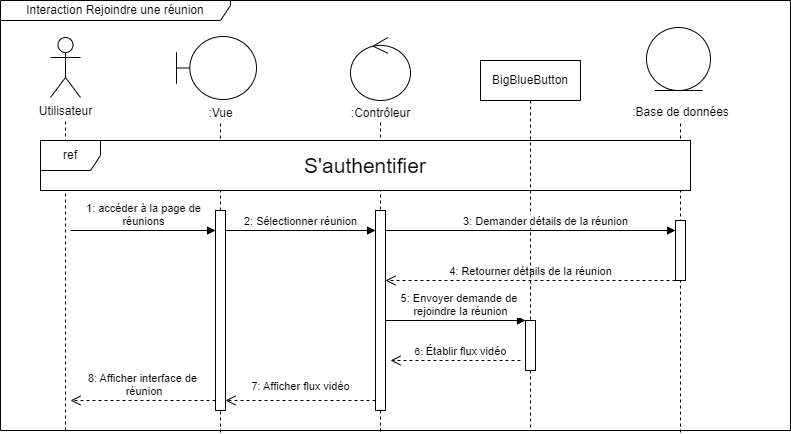
\includegraphics[width=0.8\textwidth]{images/Rejoindre une réunionSéquencefinale1.drawio.png}
    \caption{Diagramme de séquence Rejoindre une réunion}
    \label{fig:rejoindre_une_réunion_seq}
\end{figure}
\subsubsection{Diagramme de séquence de "Gérer les enregistrements de réunions"}
La figure 6.6 présente le diagramme de séquence du cas d'utilisation "Gérer les enregistrements de réunions".

% Insérer ici l'image du diagramme de séquence
\begin{figure}[H]
    \centering
    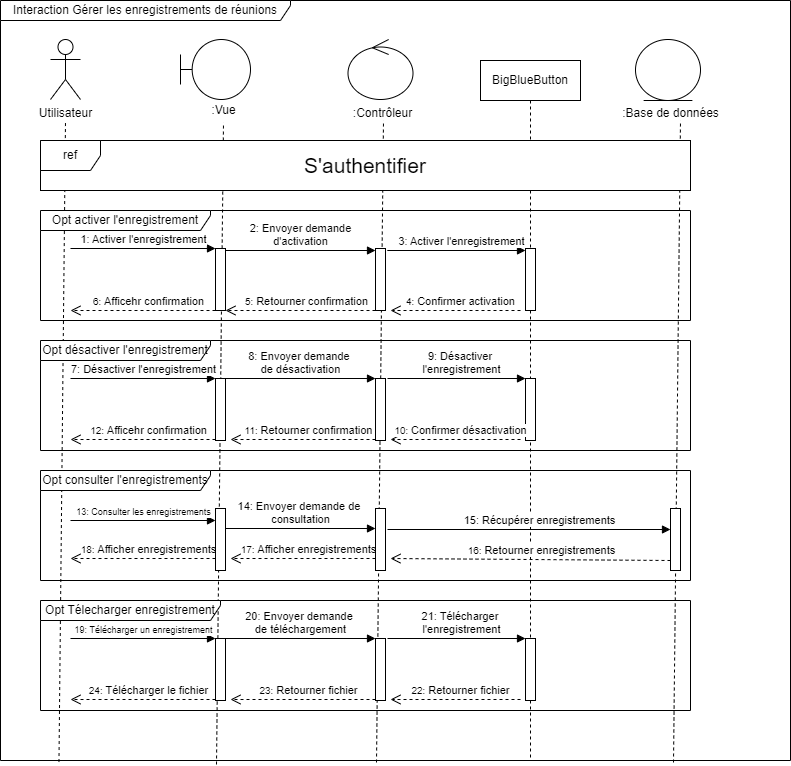
\includegraphics[width=0.8\textwidth]{images/GérerEnregistrementsRéunionsSéquencefinale1.drawio.png}
    \caption{Diagramme de séquence Gérer les enregistrements de réunions}
    \label{fig:gérer_enregistrements_réunion_seq}
\end{figure}
\section{Réalisation du sprint 6}
\subsection{Architecture générale}
Pour la réalisation du sprint 6, nous avons conservé l'architecture microservices mise en place dans les sprints précédents, en y ajoutant un nouveau microservice dédié à la gestion des réunions vidéo. Ce service s'intègre avec les services existants d'authentification et de notification pour assurer une expérience utilisateur cohérente et sécurisée.

L'architecture du système de réunions repose sur une combinaison de technologies synchrones (WebRTC pour les flux vidéo en temps réel) et asynchrones (WebSockets pour les notifications et signaux de contrôle). Un service de stockage dédié est également implémenté pour la gestion des enregistrements vidéo.

\subsection{Réalisation du module de Réunions Vidéo}
Le module de réunions vidéo a été implémenté avec un microservice dédié qui gère l'ensemble du cycle de vie des réunions, depuis leur création jusqu'à l'archivage des enregistrements. Les principales fonctionnalités développées incluent :

\begin{itemize}
    \item La création et planification de réunions avec paramètres personnalisables
    \item Le système d'invitation et gestion des participants
    \item Le moteur de streaming vidéo en temps réel basé sur BBB(Big Blue Button)
    \item L'enregistrement et stockage sécurisé des sessions
    \item Le partage de présentations et documents pendant les réunions
    \item Le système de notifications et rappels automatiques
    \item La génération de statistiques et rapports de participation
\end{itemize}

La mise en œuvre technique a nécessité l'intégration de plusieurs technologies spécialisées :

\begin{itemize}
    \item Un serveur de signalisation pour établir les connexions basé sur BBB(Big Blue Button)
    \item Des serveurs TURN et STUN pour faciliter les connexions à travers les NAT et pare-feux basé sur BBB(Big Blue Button)
    \item Un système de gestion de médias (microservice média) pour l'enregistrement, le traitement et le stockage des vidéos
    \item Une API de planification pour la gestion des réunions futures et des rappels intégres avec le microservice notfication et BBB(Big Blue Button)
    \item Une interface utilisateur réactive et optimisée pour les interactions en temps réel
\end{itemize}

\subsection{Intégration de BigBlueButton}
Pour implémenter notre système de réunions vidéo, nous avons fait le choix d'intégrer BigBlueButton, une solution open-source robuste spécialisée dans les conférences web. Cette décision s'inscrit dans notre stratégie d'utiliser des technologies éprouvées pour les fonctionnalités critiques, tout en les intégrant parfaitement dans notre écosystème applicatif.

\subsubsection{Présentation de BigBlueButton}
BigBlueButton est une plateforme de visioconférence open-source conçue spécifiquement pour l'apprentissage en ligne et la collaboration à distance. Elle offre un ensemble complet de fonctionnalités essentielles pour notre service de réunions :

\begin{itemize}
    \item Partage audio et vidéo en temps réel avec qualité adaptative
    \item Partage d'écran et de documents multiformats
    \item Tableau blanc interactif pour la collaboration visuelle
    \item Chat public et privé pendant les sessions
    \item Sondages en direct pour recueillir des feedbacks
    \item Salles de sous-groupes pour les discussions en petits comités
    \item Enregistrement complet des sessions avec possibilité de replay
    \item Interface responsive adaptée aux différents appareils
\end{itemize}

\subsubsection{Architecture d'intégration}
L'intégration de BigBlueButton avec notre plateforme a été réalisée selon une architecture de microservices communiquant via API. La figure 6.7 illustre cette architecture d'intégration.

% Insérer ici l'image du diagramme d'architecture d'intégration

Notre approche d'intégration comprend plusieurs composants clés :

\begin{itemize}
    \item \textbf{API Gateway} : Gère l'authentification et le routage des requêtes vers le microservice de réunions.
    
    \item \textbf{Microservice Meetings} : Orchestrateur central qui :
    \begin{itemize}
        \item Communique avec l'API Greenlight de BigBlueButton
        \item Gère les métadonnées des réunions dans notre base de données
        \item Maintient la synchronisation entre notre modèle de données et BigBlueButton
        \item Implémente les règles métier spécifiques à notre application
    \end{itemize}
    
    \item \textbf{BigBlueButton API Wrapper} : Couche d'abstraction qui :
    \begin{itemize}
        \item Gère la génération sécurisée des jetons de connexion
        \item Traduit nos modèles d'objets en paramètres compatibles avec BigBlueButton
        \item Simplifie l'intégration en cachant la complexité de l'API native
    \end{itemize}
    
    \item \textbf{Service de notification} : Alerte les participants avant les réunions et lors des modifications.
    
    \item \textbf{Service de stockage} : Gère les enregistrements exportés depuis BigBlueButton.
\end{itemize}

\subsubsection{Sécurité et authentification}
La sécurité étant primordiale, nous avons mis en place un système robuste pour l'authentification et l'autorisation :

\begin{itemize}
    \item Authentification par jeton JWT pour l'accès à l'API
    \item Chiffrement TLS pour toutes les communications
    \item Mécanisme de vérification de rôle pour contrôler les droits des participants
    \item Isolation des salles de réunion pour garantir la confidentialité
\end{itemize}

\subsubsection{Personnalisation de l'interface}
Pour offrir une expérience utilisateur cohérente avec le reste de notre application, nous avons personnalisé l'interface de BigBlueButton :

\begin{itemize}
    \item Adaptation des couleurs et des éléments visuels à notre charte graphique
    \item Intégration transparente via iFrame avec communication JavaScript bidirectionnelle
    \item Simplification de certains contrôles pour une prise en main facilitée
   
\end{itemize}

\subsubsection{Déploiement et scalabilité}
Le déploiement de BigBlueButton a été réalisé avec une approche orientée haute disponibilité :

\begin{itemize}
    \item Architecture conteneurisée avec Docker pour faciliter le déploiement et la maintenance
    \item Configuration d'un cluster de serveurs BigBlueButton pour la répartition de charge
    \item Mécanismes de failover automatique en cas de défaillance d'un nœud
\end{itemize}


\subsubsection{Résultats et performances}
L'intégration de BigBlueButton a été un succès, permettant d'atteindre les performances suivantes :

\begin{itemize}
    \item Support simultané de plus de 100 salles de réunion actives
    \item Capacité de 50+ participants par réunion sans dégradation notable
    \item Latence inférieure à 200ms dans des conditions réseau normales
    \item Temps de démarrage d'une réunion inférieur à 3 secondes
    \item Disponibilité de service supérieure à 97\% sur la période de test
  
\end{itemize}

Cette intégration nous permet d'offrir une solution de réunions vidéo complète et robuste, parfaitement intégrée à notre plateforme, tout en bénéficiant de la maturité et de la richesse fonctionnelle de BigBlueButton.

\section{Technologies et Outils Utilisés}
Cette section présente les principales technologies et outils utilisés pour la réalisation du sprint 6, notamment pour le développement du système de réunions vidéo.

\vspace{0.5cm} %
\begin{tabular}{| m{2.5cm} | m{13cm} |}
\hline

\includegraphics[width=2cm]{images/sha1.png} & 
\textbf{SHA-1 : \cite{sha1}}  
Algorithme de hachage cryptographique utilisé pour générer les signatures nécessaires aux appels API sécurisés vers BigBlueButton.
\\
\hline

\end{tabular}
\vspace{0.5cm} % Espace entre les deux tableaux

\begin{tabular}{| m{2.5cm} | m{13cm} |}
\hline


\includegraphics[width=2cm]{images/BigBlueButton.png} & 
\textbf{BigBlueButton : \cite{bigbluebutton}}  
Plateforme open-source de visioconférence que nous avons intégrée comme solution principale pour les réunions vidéo. Elle fournit les fonctionnalités essentielles telles que le partage d'écran, le chat en temps réel, le tableau blanc collaboratif et l'enregistrement des sessions.
\\
\hline


\includegraphics[width=2cm]{images/webrtc.png} & 
\textbf{WebRTC : \cite{webrtc}}  
Technologie sous-jacente utilisée par BigBlueButton pour la communication audio/vidéo en temps réel entre les participants. Cette norme ouverte permet des communications peer-to-peer sécurisées directement dans le navigateur.
\\
\hline


\includegraphics[width=2cm]{images/joi.png} & 
\textbf{Joi : \cite{joi}}  
Bibliothèque de validation de schéma pour JavaScript, utilisée pour valider les données de réunion avant leur traitement par le serveur.
\\
\hline


\includegraphics[width=2cm]{images/jest.png} & 
\textbf{Jest : \cite{jest}}  
Framework de test JavaScript utilisé pour les tests unitaires et d'intégration du microservice de réunions, assurant la fiabilité des fonctionnalités développées.
\\
\hline

\end{tabular}


\section{Présentation des interface de l'application}
\newpage
\begin{figure}[H]
    \centering

    % Top row: two mobile screenshots side by side
    \begin{minipage}[b]{0.45\textwidth}
        \centering
        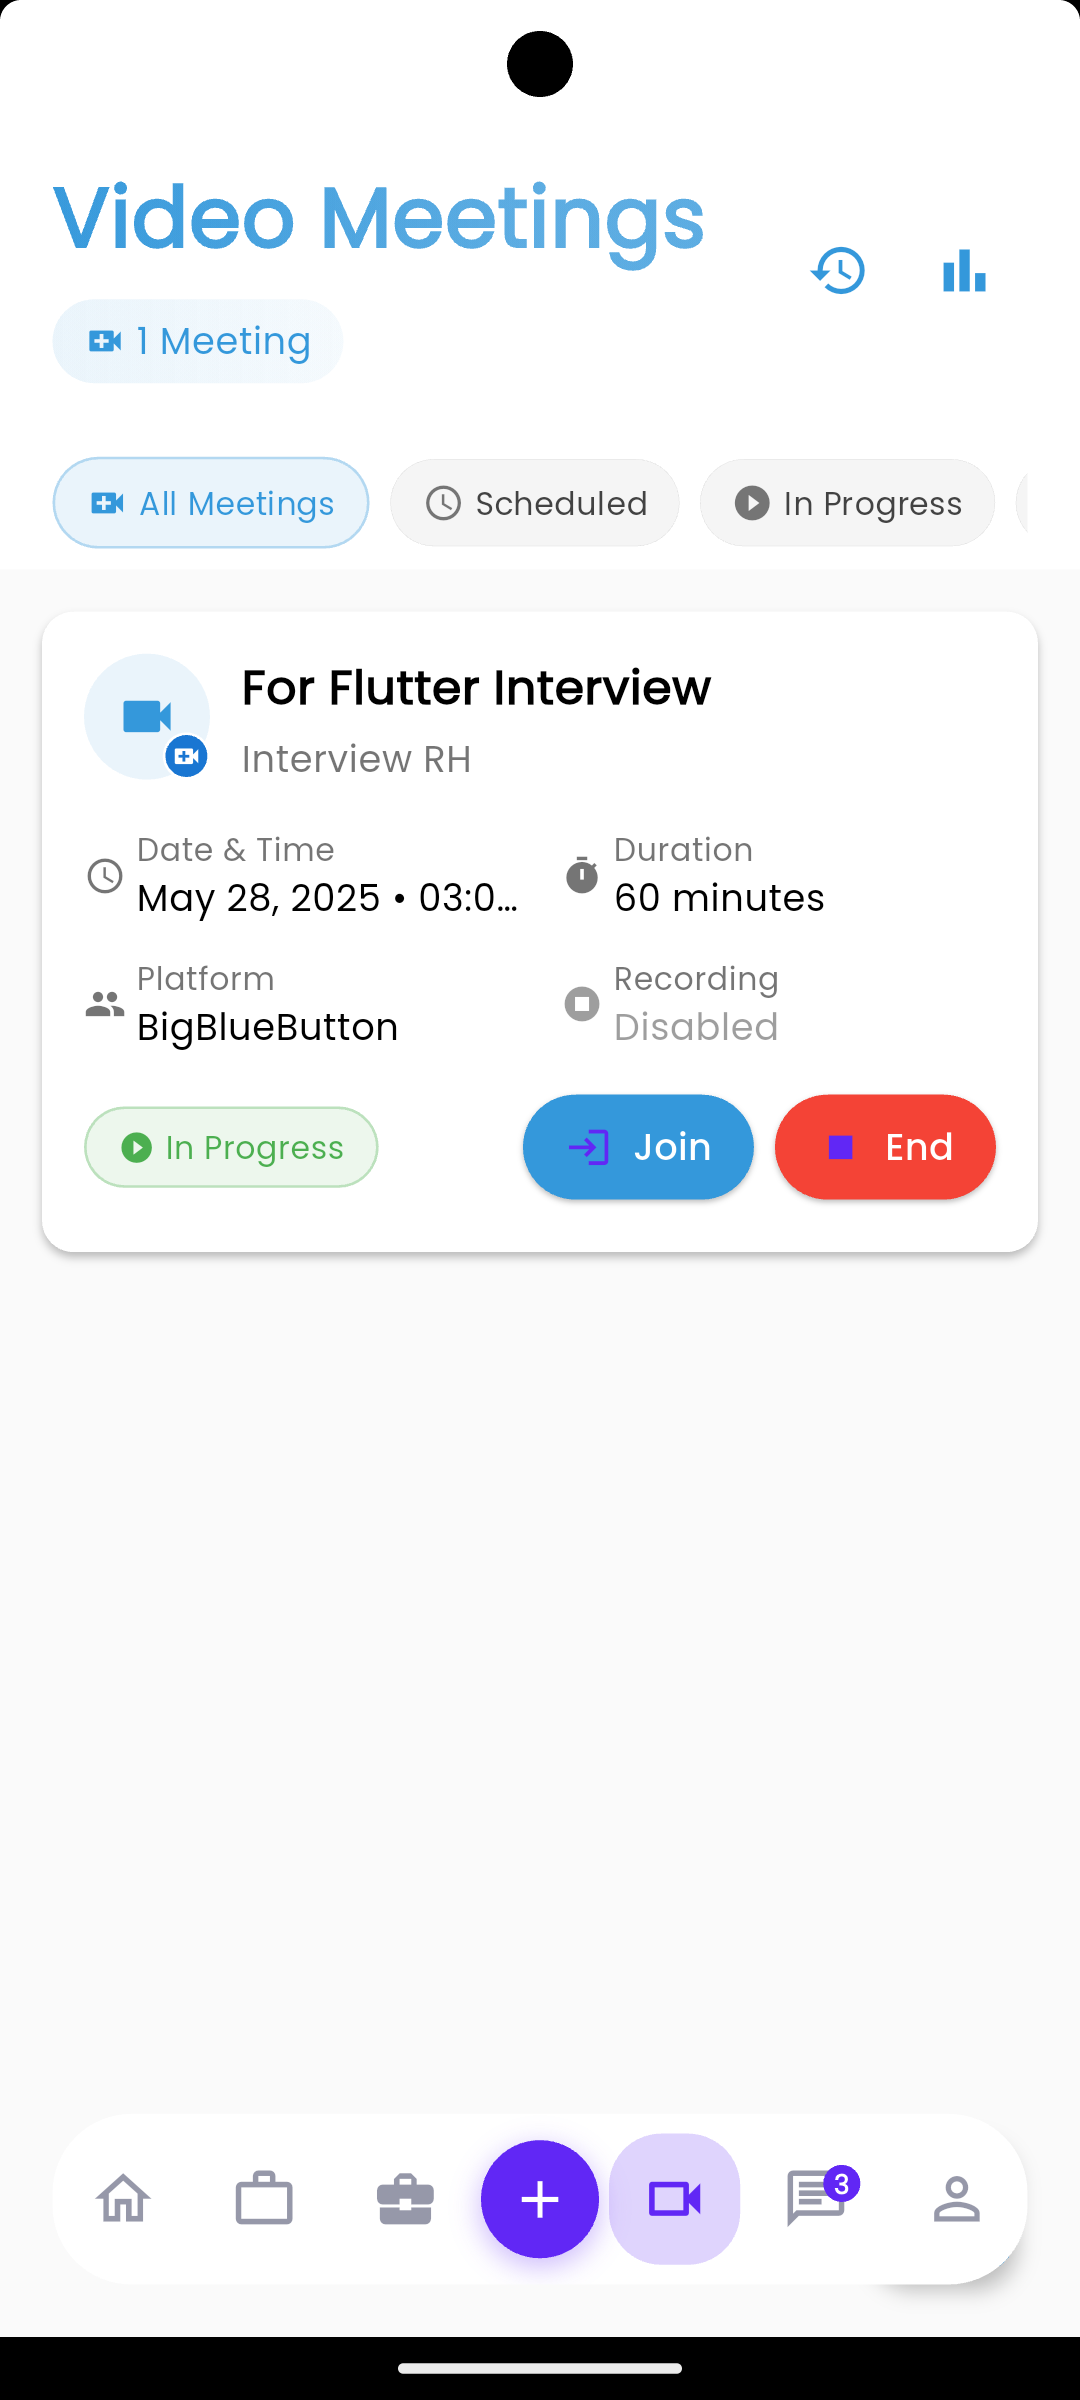
\includegraphics[width=0.8\linewidth, keepaspectratio]{images/PageJoinmeeting.png}
        \caption{Interface Mobile – Page Créer \& rejoindre réunion – étape 1}
    \end{minipage}
    \hfill
    \begin{minipage}[b]{0.45\textwidth}
        \centering
        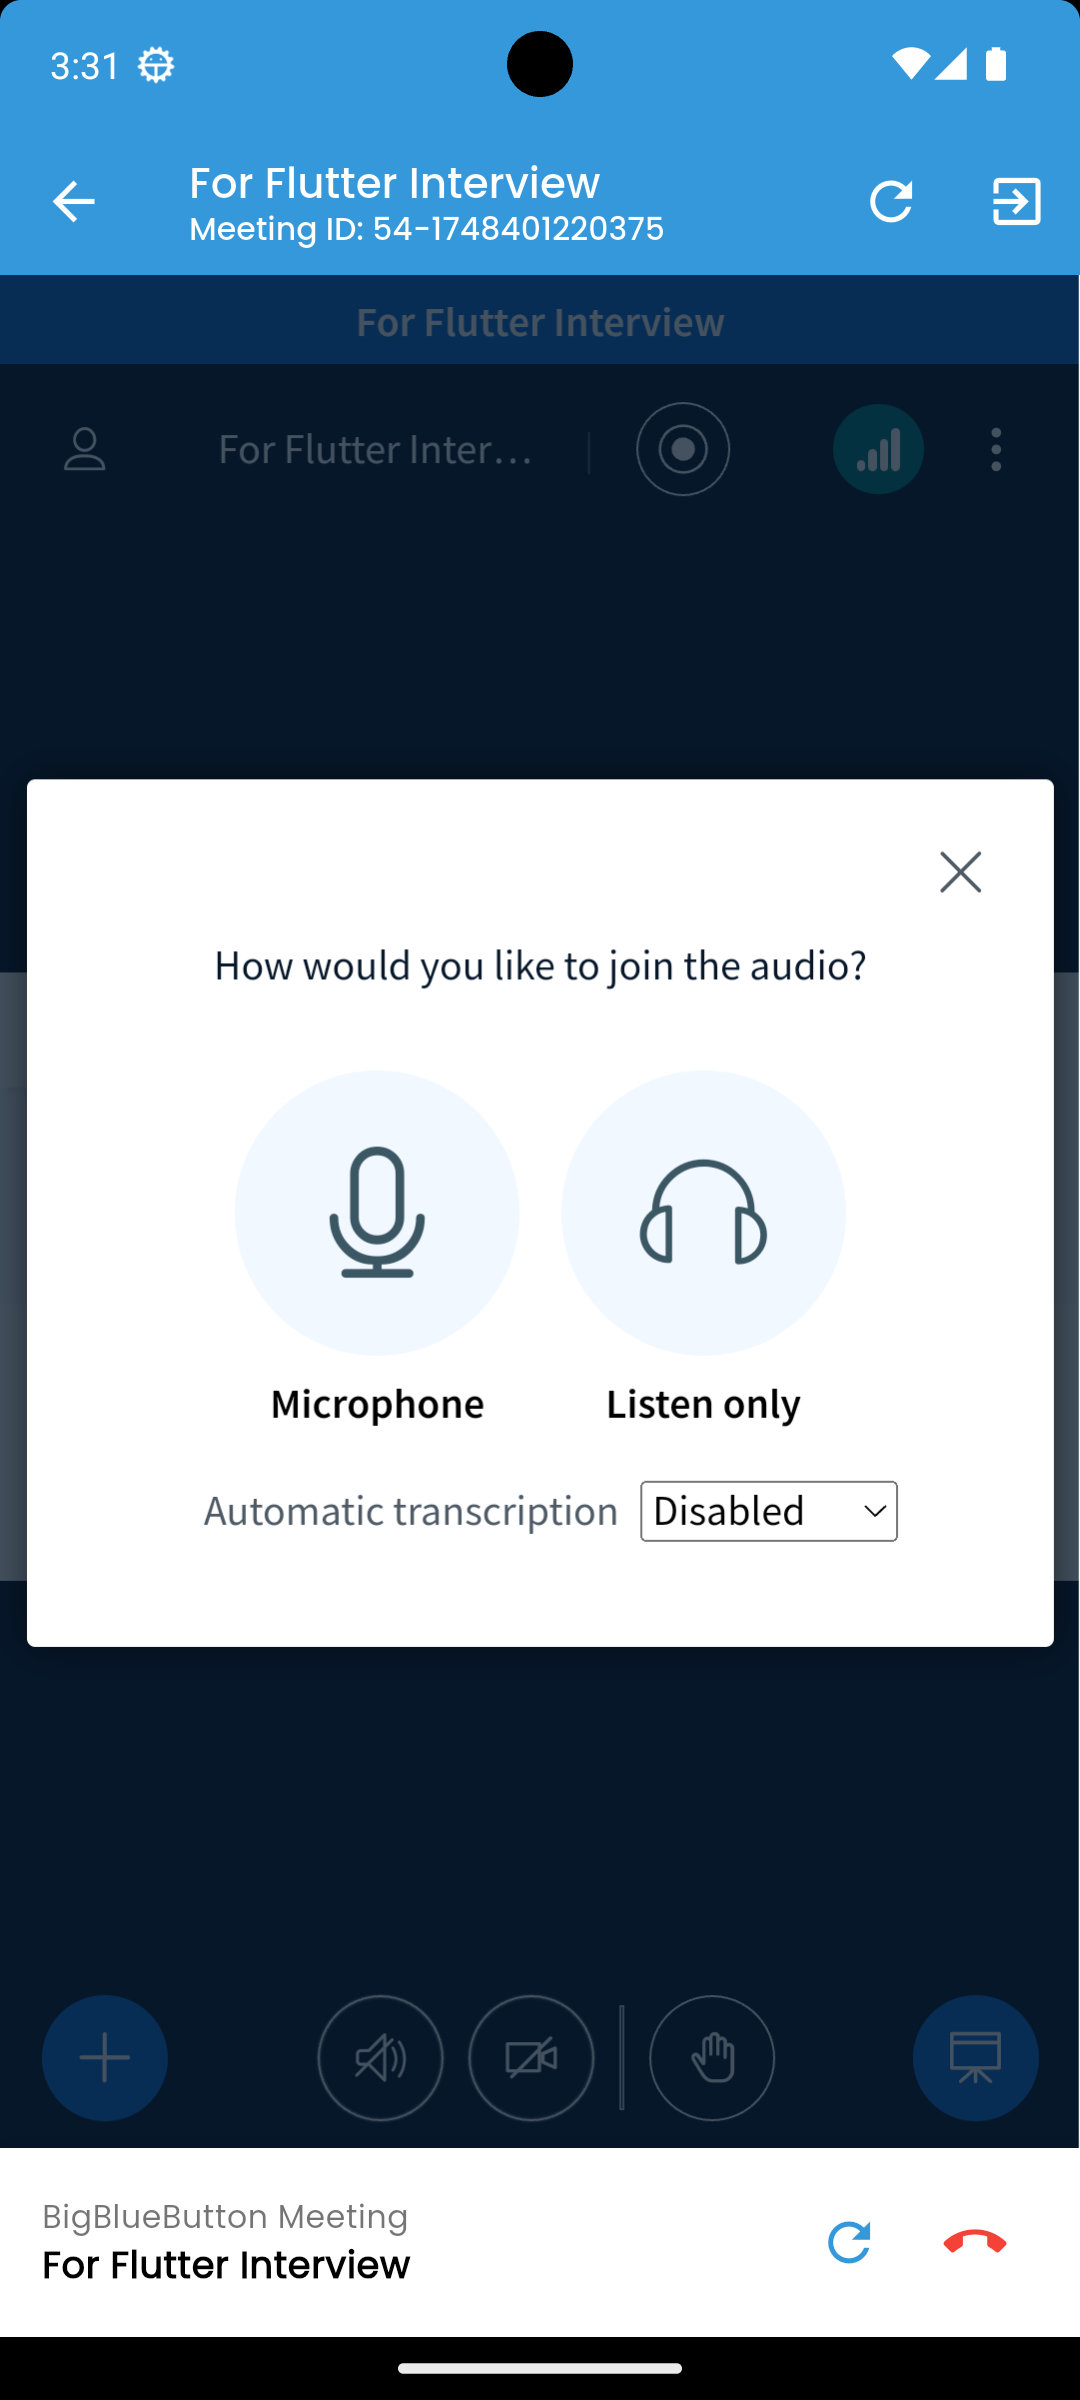
\includegraphics[width=0.8\linewidth, keepaspectratio]{images/joinmeeting.png}
        \caption{Interface Mobile – Joindre réunion – étape 2}
    \end{minipage}

    \vspace{1em}

    % Bottom: web interface full width with height limit
    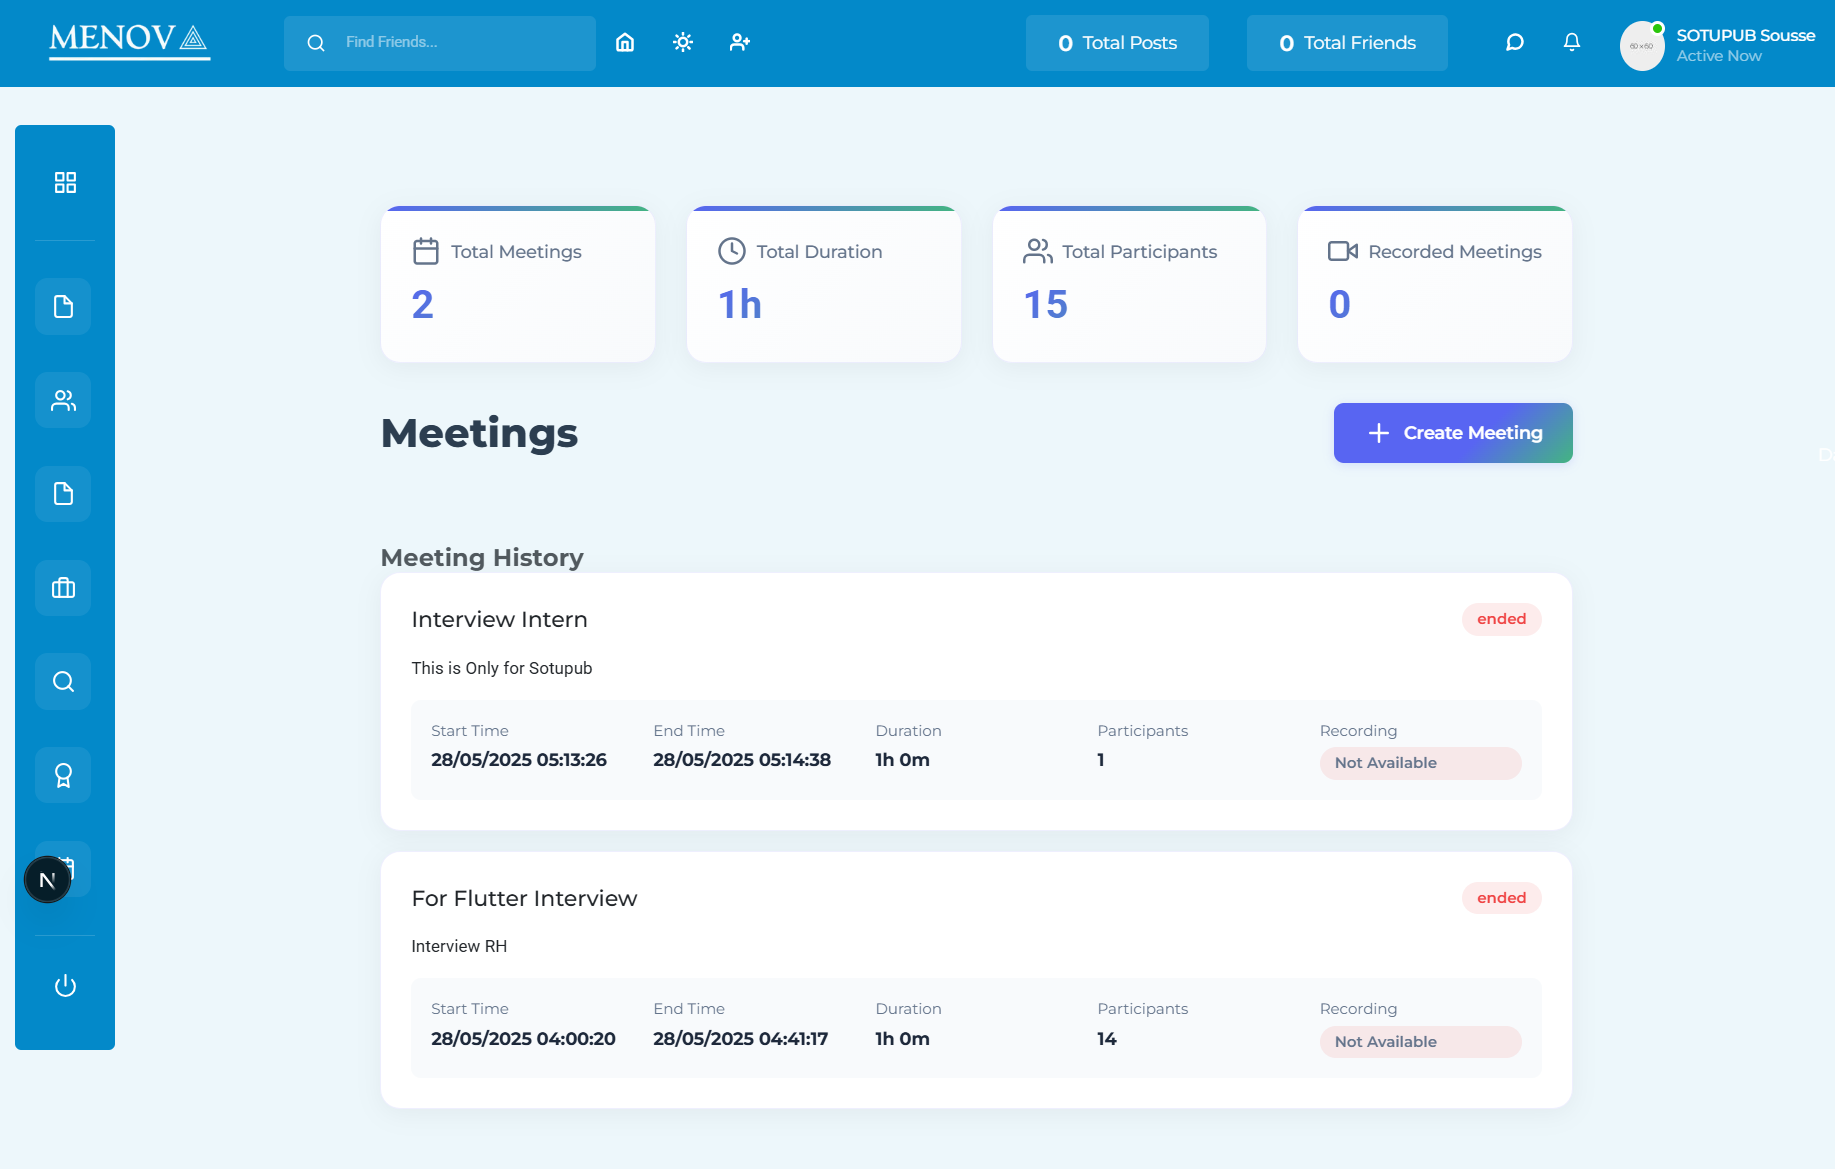
\includegraphics[width=0.9\textwidth, height=0.35\textheight, keepaspectratio]{images/meetingHistory.png}
    \caption{Interface Web – Historique \& Statistiques de réunions – étape 3}

    \label{fig:mobile-top-web-bottom}
\end{figure}

      \newpage


\section*{Conclusion}
\addcontentsline{toc}{section}{Conclusion}
Le sprint 6 a permis d'enrichir notre plateforme avec un système complet de réunions vidéo, offrant aux utilisateurs la possibilité d'organiser et participer à des sessions collaboratives directement depuis l'application. Cette fonctionnalité répond à un besoin essentiel de communication en temps réel dans un contexte professionnel de plus en plus orienté vers le travail à distance.

Les fonctionnalités avancées comme l'enregistrement des sessions, le partage de présentations et les statistiques de participation positionnent notre solution comme une alternative crédible aux outils de visioconférence spécialisés, avec l'avantage d'une intégration native à notre écosystème collaboratif.

Les développements réalisés durant ce sprint constituent une étape importante dans la transformation de notre application en une plateforme complète de collaboration professionnelle, combinant communication asynchrone (messagerie) et synchrone (réunions vidéo) au sein d'un environnement unifié. 